\begin{figure}[h!]
\begin{center}
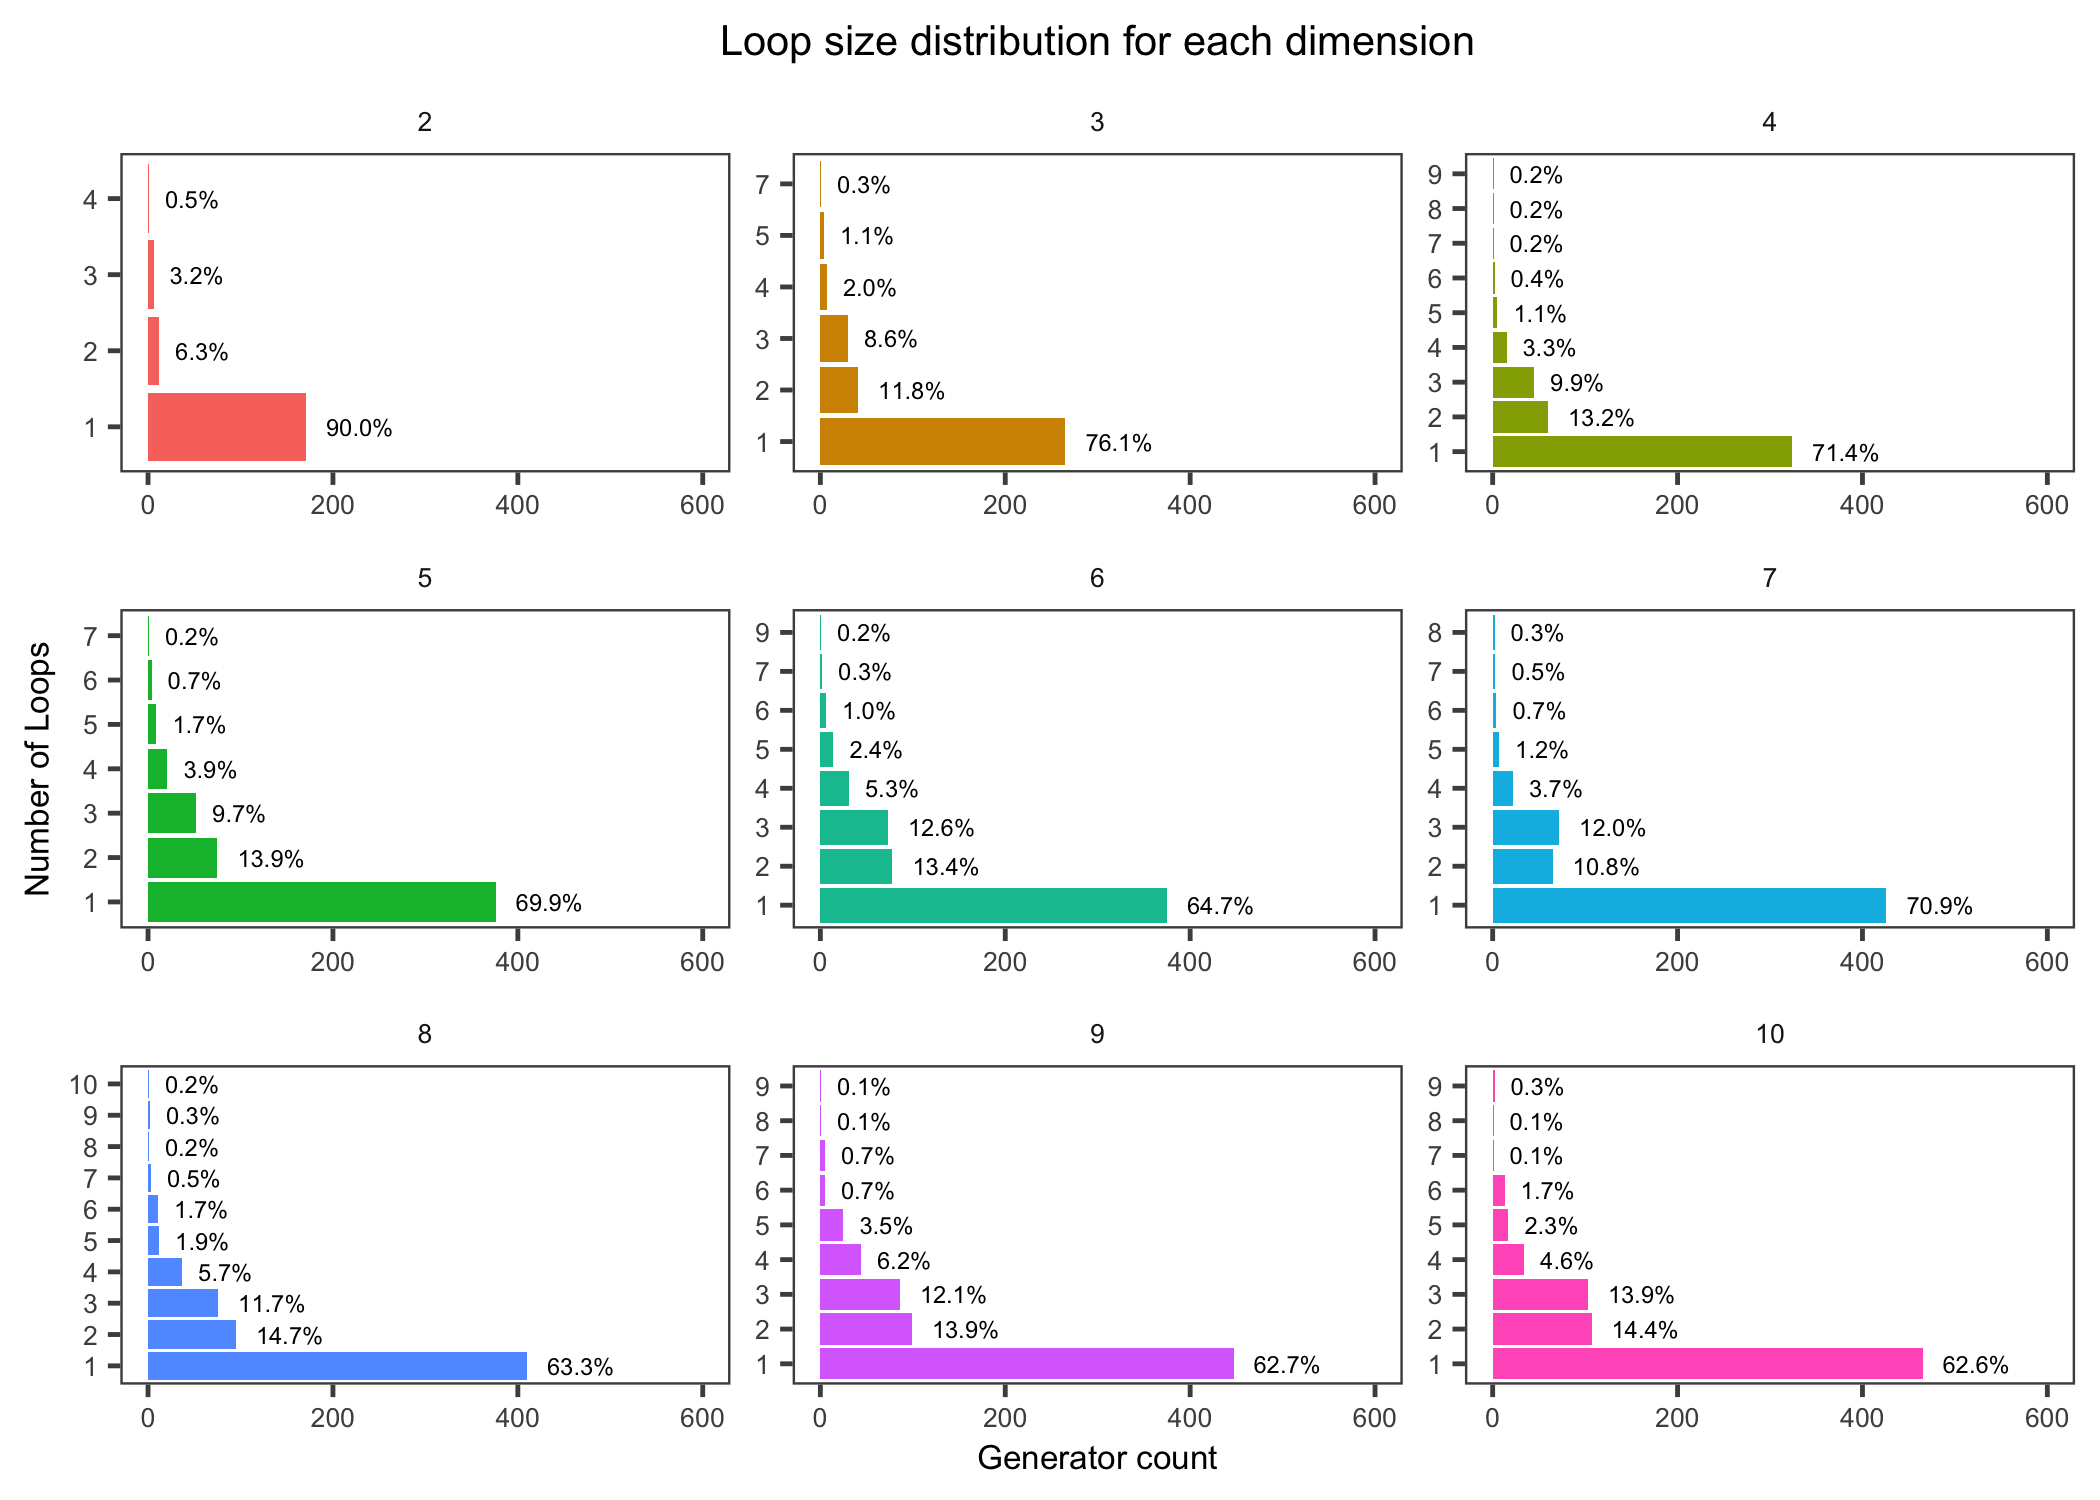
\includegraphics[width=\textwidth]{figures/loopsBreakdown.png}
\end{center}
\caption{%\GHP{First betti number of the support of $\optimalrep$, for various 1-d cycle representatives $\optimalrep$ (equivalently, the nullity of the column submatrix $[\partial_1][:, S]$, where $S = \{i : \optimalrep_i \neq 0\}$ is the support of $\optimalrep$)}\LL{Thanks for this definition, Greg! We added it to the results section 6.8. Should we also keep it here?}  
Number of loops in the original cycle representatives of each dimension (subfigure title) in the $360$ randomly generated distribution data sets. The horizontal axis is the number of representatives and the vertical axis is the number of loops in the original representative. We observe that original cycle representatives can have up to 10 loops in higher dimensions, and in general, it is not uncommon to find an original representative with multiple loops.} \label{fig:loopsbreakdown}
\end{figure} 
% 